\documentclass[12pt, a4paper]{article}

\usepackage[utf8]{inputenc}
\usepackage[T1]{fontenc}
\usepackage[russian]{babel}
\usepackage[oglav,spisok,boldsect, figwhole]{./style/fn2kursstyle1}
\graphicspath{{./style/}{./figures/}}
%\usepackage{float}%"Плавающие" картинки
\usepackage{multirow}
\usepackage{subcaption}
\usepackage{float}%"Плавающие" картинки
%Римские цифры
\newcommand{\RomanNumeralCaps}[1]
{\MakeUppercase{\romannumeral #1}}

\usepackage{enumitem} 
\usepackage{amsmath}
\usepackage{comment}
\usepackage{makecell}

%Параметры титульника
\title{Численное решение краевых задач для двумерного уравнения Пуассона}
\group{ФН2-62Б}
\author{З.И.~Абрамов, Г.А.~Швецов}
\supervisor{С.А.~Конев}
\date{2023}
\begin{document}
	\newcommand{\pl}{\partial}
	\maketitle
	
	\tableofcontents
	
	\newpage
	
	\section{Контрольные вопросы}
	\begin{enumerate}
		\item \textit{Оцените число действий, необходимое для перехода на следующий слой по времени методом переменных направлений.}
		\smallskip
		
		Выпишем первые этапы метода переменных направлений в случае граничных условий I рода:
		\begin{eqnarray*}
			&F(y) = \dfrac2\tau y + \Lambda_2 y + \varphi, \quad F^k_{ij} = F(y^k_{ij}),\\
			&\dfrac1{h_1^2} y^{k+1/2}_{i-1,j} - 2 \left(\dfrac1{h_1^2} + \dfrac1\tau\right) y^{k+1/2}_{ij} + \dfrac1{h_1^2} y^{k+1/2}_{i+1,j} = -F^k_{ij},\\
			&u_{0,j} = \Omega_{0,j}, \quad u_{N_1,j} = \Omega_{N_1,j}, \quad j = 1, 2, \dots, N_2 -1.
		\end{eqnarray*}
		Для вычисления $F^k_{ij}$ требуется порядка $3 N_1 N_2$ умножений. 2 и 3 строки представляет собой $N_2-1$ трехдиагональных СЛАУ размерности $N_1 - 1$. Для их решения требуется примерно $5 N_1 N_2$ операций. Такой же порядок операций получается и для остальных этапов:
		\begin{eqnarray*}
			&\hat{F}(y) = \dfrac2\tau y + \Lambda_1 y + \varphi, \quad \hat{F}^{k+1/2}_{ij} = \hat{F}(y^{k+1/2}_{ij}),\\
			&\dfrac1{h_2^2} y^{k+1}_{i,j-1} - 2 \left(\dfrac1{h_2^2} + \dfrac1\tau\right) y^{k+1}_{ij} + \dfrac1{h_2^2} y^{k+1}_{i,j+1} = -\hat{F}^{k+1/2}_{ij},\\
			&u_{i,0} = \Omega_{i,0}, \quad u_{i,N_2} = \Omega_{i,N_2}, \quad i = 1, 2, \dots, N_1 -1.
		\end{eqnarray*}
		Таким образом, для перехода на следующий слой по времени требуется порядка $16 N_1 N_2$ операций.
		
		\item \textit{Почему при увеличении числа измерений резко возрастает количество операций для решения неявных схем (по сравнению с одномерной схемой)?}
		\smallskip
		
		При повышении размерности увеличивается размерность $F$, т.е. увеличивается количество операций, причем во столько раз, сколько узлов $N_n$ по добавленной размерности, а также количество таких элементов $F$. Также увеличивается сложность прогонки в такое же количество раз. Таким образом, количество операций составляет $O(N_1 \dots N_n)$, где $n$ --- размерность пространства, что резко увеличивает сложность перехода к новому временному слою, $N_i$ --- количество узлов по каждой координатной оси.
		
		\item \textit{Можно ли использовать метод переменных направлений в областях произвольной формы?}
		\smallskip
		
		Да, метод переменных направлений достаточно просто использовать в случае области произвольного вида. Основное отличие от прямоугольной области будет состоять в том, что при решении СЛАУ для $y^{k+1/2}_{ij}$ диапазон изменения индекса $i$ будет не константным, а зависеть от $j$. Также при нахождении $y^{k+1}_{ij}$ диапазон $j$ будет зависеть от $i$.
		
		% TODO как-то коротко
		
		\item \textit{Можно ли использовать метод переменных направлений для решения пространственных и вообще n-мерных задач?}
		\smallskip
		
		Продольно-поперечная схема на задачи с $p \ge 3$ непосредственно не обобщается вследствие возникающих несимметричности и условной устойчивости. Имевшаяся в двумерном случае симметричность давала равные (по модулю) ошибки с разными знаками на двух последовательных шагах, компенсировавшие друг друга.
		
		Однако в этом случае можно использовать локально-одномерную схему также с использованием промежуточных (дробных) слоев. Эта схема имеет лишь суммарную аппроксимацию, а на промежуточных слоях она не аппроксимирует исходное дифференциальное уравнение. Однако ошибки аппроксимации при суммировании гасят друг друга. Так что решение на <<целом>> слое оказывается приближением точного. Ее запись приведена в дополнительном вопросе <<Трехмерный случай>>.
		
		\item \textit{Можно ли использовать метод переменных направлений на неравномерных сетках?}
		\smallskip
		
		Метод переменных направлений невозможно использовать на неравномерных сетках, так как в этом случае невозможно выделить эти самые направления.
		
		% TODO как-то очень коротко
		
	\end{enumerate}
	\newpage
	
	\section{Дополнительные вопросы}
	\begin{enumerate}
		\item \textit{Монотонность. Выведите условия положительности коэффициентов для схемы переменных направлений.}
		\smallskip
		
		Схема записывается следующим образом:
		\begin{eqnarray*}
			& \dfrac2\tau y^{k+1/2} - \Lambda_1 y^{k+1/2} = \dfrac2\tau y^k + \Lambda_2 y^k + \varphi, \\
			& \dfrac2\tau y^{k+1} - \Lambda_2 y^{k+1} = \dfrac2\tau y^{k+1/2} + \Lambda_1 y^{k+1/2} + \varphi.
		\end{eqnarray*}
		
		Вычтем первое выражение из второго и выразим $y^{k+1/2}$:
		\begin{eqnarray*}
			& \dfrac2\tau y^{k+1} - \dfrac2\tau y^{k+1/2} - \Lambda_2 y^{k+1} + \Lambda_1 y^{k+1/2} = \dfrac2\tau y^{k+1/2} - \dfrac2\tau y^k + \Lambda_1 y^{k+1/2} - \Lambda_2 y^k, \\
			& \dfrac2\tau (y^{k+1}+y^k) - \Lambda_2 (y^{k+1}-y^k) = \dfrac4\tau y^{k+1/2},\\
			& y^{k+1/2} = \dfrac12 (y^{k+1}+y^k) - \dfrac\tau4 \Lambda_2 (y^{k+1}-y^k).
		\end{eqnarray*}
		
		Подставим во второе выражение исходной схемы и сократим слагаемые:
		\begin{equation*}
			\dfrac1\tau y^{k+1} - \dfrac12 \Lambda y^{k+1} + \dfrac\tau4 \Lambda_1 \Lambda_2 y^{k+1} = \dfrac1\tau y^k + \dfrac12 \Lambda y^k + \dfrac\tau4 \Lambda_1 \Lambda_2 y^k + \varphi,
		\end{equation*}
		где $\Lambda = \Lambda_1 + \Lambda_2$. Заметим, что узлы $y^{k+1}_{i+1, j+1}$, $y^{k+1}_{i+1, j-1}$, $y^{k+1}_{i-1, j+1}$ и $y^{k+1}_{i-1, j-1}$ указаны только лишь в слагаемом вида $\Lambda_1 \Lambda_2 y^{k+1}$. Распишем его:
		\begin{multline*}
			\Lambda_1 \Lambda_2 y^{k+1} = \Lambda_1 \left(\dfrac{y^{k+1}_{i,j+1} - 2 y^{k+1}_{i,j} + y^{k+1}_{i,j-1}}{h_2^2}\right) = \dfrac1{h_2^2}\left( \Lambda_1 y^{k+1}_{i,j+1} - 2 \Lambda_1 y^{k+1}_{i,j} + \Lambda_1 y^{k+1}_{i,j-1}\right) = \\
			%
			= \dfrac1{h_1^2 h_2^2} \Big(y^{k+1}_{i+1,j+1} -2 y^{k+1}_{i,j+1}+y^{k+1}_{i-1,j+1} - 2 (y^{k+1}_{i+1,j} - 2 y^{k+1}_{i,j} + y^{k+1}_{i-1,j}) + y^{k+1}_{i+1,j-1} - 2 y^{k+1}_{i,j-1} + y^{k+1}_{i-1,j-1}\Big).
		\end{multline*}
		Видно, что коэффициенты при указанных узлах положительны. Таким образом, после переноса их направо они станут отрицательными. Также можно показать, что коэффициенты при $y^{k+1}_{i, j+1}$, $y^{k+1}_{i, j-1}$, $y^{k+1}_{i-1, j}$ и $y^{k+1}_{i-1, j}$ будут положительными, т.е. условие положительности коэффициентов в любом случае не выполняется.
		
		\item \textit{Критерий останова. Какой критерий останова Вы использовали в счете на установление?}
		\smallskip
		
		Наиболее простым критерием останова является выполнение условия
		\[
		\|\hat{y} - y\| \le \varepsilon;
		\]
		однако он недостаточно надежен, поскольку разностное решение устанавливается медленно.
		
		Можно показать\cite{kalitkin}, что разность решений уравнения теплопроводности и уравнения Пуассона экспоненциально стремится к нулю по норме $\|\phantom{1}\|_{L_2}$ при $t\rightarrow\infty$. Таким образом, установление происходит почти по геометрической прогрессии, и можно получить более надежный критерий:
		\[
		\|\hat{y}-y\| \le \varepsilon (1-\nu), \quad \text{ где } \nu = \frac{\|\hat{y}-y\|}{\|y-\check{y}\|}.
		\]
		
		Этот критерий и был реализован в нашей программе.
		
		\item \textit{Трехмерный случай. Обобщите продольно-поперечную схему на трехмерный случай. Предоставьте запись схемы.}
		\smallskip
		
		Для многомерного случая обобщением продольно-поперечной схемы является локально-одномерная схема. Рассмотрим уравнение
		\[
		u_t = \sum_{i = 1}^p u_{x_i x_i} + f.
		\]
		
		Аппроксимируем это уравнение, используя симметричную неявную схему
		\[
		y_t = \sum_{i = 1}^p \Lambda_i y^{(0,5)} + \varphi,
		\]
		($\Lambda_i$ --- разностная вторая производная по координате $x_i$).
		
		Наряду с исходной схемой построим локально-одномерную схему. Для этого между слоями $t$ и $\hat t$ введем $p + 1$ промежуточных слоев с шагами $\tau / p$ между ними. Первый слой соответствует моменту времени $t$, последний с номером $p+1$ --- моменту времени $\hat t$. На каждом таком слое с номером $\alpha$ суммарный оператор в правой части заменим оператором $\Lambda_\alpha$. Обозначим решение на промежуточных шагах через $w_\alpha$, $\alpha = 1, 2, \dots, p$. Тогда $w_\alpha$ является решением следующей разностной задачи:
		\begin{eqnarray*}
			& \dfrac1\tau (\hat w_\alpha - w_\alpha) = \dfrac12 \Lambda_\alpha(\hat w_\alpha + w_\alpha) + \varphi_\alpha, \quad \alpha = 1, 2, \dots, p; \\
			& w_1 = y, w_2 = \hat w_1, \dots, w_p = \hat w_{p-1}, \hat w_p = \hat y.
		\end{eqnarray*}
		
		Очевидно, что для любого $p$ соответствующее уравнение является одномерным, решаемым методом обычной прогонки. Остальные независимые переменные участвуют в нем только в качестве параметров. Поэтому и схема называется локально-одномерной.
		
		\item \textit{Порядок сходимости. Покажите, что рассматриваемая схема имеет порядок сходимости, предсказываемый теорией (составьте таблицу погрешностей и порядков сходимости в зависимости от шагов $\tau$, $h_1$ и $h_2$).}
		\smallskip
		
		Метод переменных направлений обладает квадратичной скоростью сходимости по времени и пространству, т.е. $O(\tau^2+h_1^2+h_2^2)$.
		
		Для проверки порядка сходимости возьмем следующий пример уравнения теплопроводности:
		\begin{eqnarray*}
			& u_t = \mathcal{4}u, \qquad (x_1, x_2) \in [0, 2]\times [0, 1],\\
			& u\Big|_{(x_1, x_2) \in \Gamma} = 0, \qquad u(x_1, x_2, 0) = \sin\left(\dfrac{\pi x_1}2\right) \sin(\pi x_2),
		\end{eqnarray*}
		точное решение которого имеет вид $u = \exp\left(-\dfrac{5\pi^2}4 t\right)\sin\left(\dfrac{\pi x_1}2\right) \sin(\pi x_2)$.
		
		\begin{table}[H]
			\caption{Порядок сходимости}
			\centering
			\begin{tabular}{|c|c|c|c|}\hline
				$h_1, h_2 = h_1 / 2, \tau = 5 h_1$ & AbsErr($\tau,\,h_1, h_2$) & $\Delta$ & $\log_2 \Delta$\\ 
				\hline
				0.02 & 0.0265178 & --- & --- \\
				\hline
				0.01 & 0.00607478 & 4.36523 & 2.12606\\
				\hline
				0.005 & 0.00152092 & 3.99415 & 1.99789 \\
				\hline
				0.0025 & 0.000370375 & 4.10643 & 2.03788 \\
				\hline
				0.00125 & 9.36522e-05 & 3.9548 & 1.9836 \\
				\hline
				0.000625 & 2.35981e-05 & 3.96863 & 1.98864 \\
				\hline
			\end{tabular}
		\end{table}
		
		\item \textit{Время выхода на стационар. Как в зависимости от $\tau$ меняется время выхода решения на стационар?}
		\smallskip
		
		Для поиска времени выхода на стационар возьмем следующий пример:
		\begin{eqnarray*}
			& \mathcal{4}u = 0, \quad (x_1, x_2) \in [0, 4]\times [0, 2],\\
			& u\Big|_{x_2 = 0} = 6 - \dfrac34 x_1, \quad u\Big|_{x_2 = 2} = 3 - \dfrac34 x_1,\\
			& u\Big|_{x_1 = 0} = 6 - \dfrac32 x_2, \quad u\Big|_{x_1 = 4} = 3 - \dfrac32 x_2,
		\end{eqnarray*}
		точное решение которого имеет вид $u = 6 - \dfrac34 x_1 - \dfrac32 x_2$.
		
		В качестве шагов по пространству возьмем $h_1 = 0.02$, $h_2 = 0.01$, точность $\varepsilon = 0.01$.
		
		\begin{table}[H]
			\caption{Время выхода на стационар}
			\centering
			\begin{tabular}{|c|c|c|}\hline
				$\tau$ & Количество временных слоев & Время выхода на стационар\\ 
				\hline
				0.02 & 283 & 5.66 \\
				\hline
				0.01 & 269 & 2.69 \\
				\hline
				0.005 & 181 & 0.905 \\
				\hline
				0.0025 & 174 & 0.435 \\
				\hline
				0.00125 & 196 & 0.245 \\
				\hline
			\end{tabular}
		\end{table}
		
	\end{enumerate}
	
	\newpage
	\section{Результаты}
	\paragraph{Тестовая задача 1}
	\begin{eqnarray*}
		\Delta u=0,\quad(x_1,x_2)\in G=[0,1]\times[0,1],\\
		u(x_1,x_2)=1,\quad (x_1,x_2)\in \pl G.
	\end{eqnarray*}
		Точное решение $u(x_1,x_2)=1$.
		
		\textbf{Численное решение} $$L_1=1.0,\,L_2=2.0,\,h_1=0.001,\,h_2=0.001,\,eps=1e-3,\,\tau=0.1$$
			\begin{figure}[H]
			\centering
			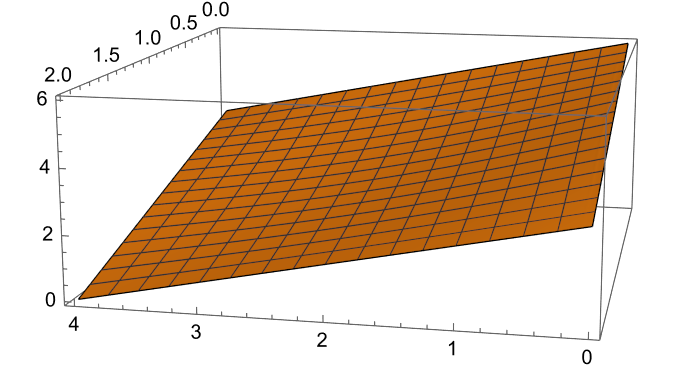
\includegraphics[width=0.7\linewidth]{test1.png}
		\end{figure}
		\paragraph{Тестовая задача 2}
		\begin{eqnarray*}
			\Delta u=0,\quad(x_1,x_2)\in G=[0,1]\times[0,1],\\
			\left.\frac{\pl u}{\pl n}\right|_{x_2=0}=-1,\quad\left.\frac{\pl u}{\pl n}\right|_{x_2=1}=1,\\
			u|_{x_1=0}=1+x_2,\quad u|_{x_1=0}=1+x_2.
		\end{eqnarray*}
		Точное решение $u(x_1,x_2)=1+x_2$.
		
		\textbf{Численное решение} $$L_1=1.0,\,L_2=2.0,\,h_1=0.001,\,h_2=0.001,\,eps=1e-3,\,\tau=0.1$$
		\begin{figure}[H]
			\centering
			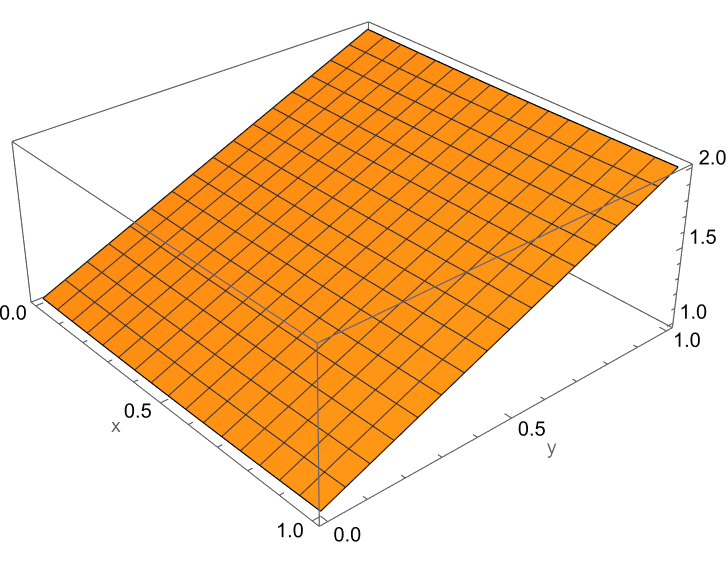
\includegraphics[width=0.7\linewidth]{test2.png}
		\end{figure}
		\paragraph{Тестовая задача 3}
		\begin{eqnarray*}
			\Delta u=4,\quad(x_1,x_2)\in G=[0,1]\times[0,1],\\
			\left.\frac{\pl u}{\pl n}\right|_{x_1=0}=0,\quad\left.\frac{\pl u}{\pl n}\right|_{x_1=1}=2,\\
			u|_{x_2=0}=x_1^2,\quad u|_{x_2=1}=1+x_1^2.
		\end{eqnarray*}
		Точное решение $u(x_1,x_2)=x_1^2+x_2^2$.
		
		\textbf{Численное решение} $$L_1=1.0,\,L_2=2.0,\,h_1=0.001,\,h_2=0.001,\,eps=1e-3,\,\tau=0.1$$
		\begin{figure}[H]
			\centering
			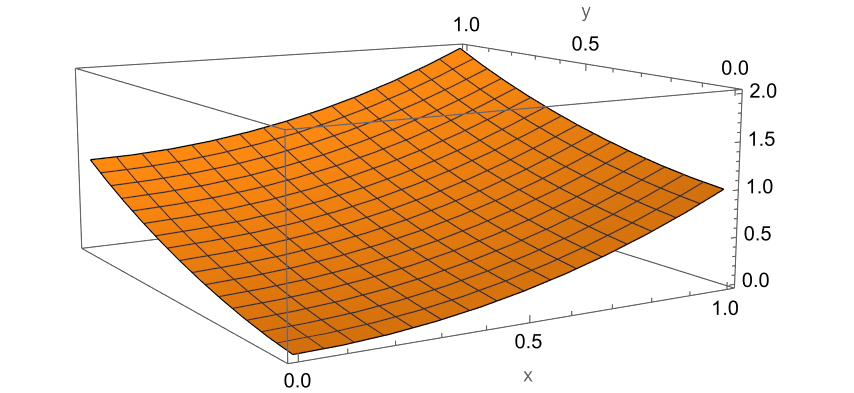
\includegraphics[width=0.7\linewidth]{test3.png}
		\end{figure}
	
		\paragraph{Тестовая задача 4 (наш тест)}
	\begin{eqnarray*}
		& \mathcal{4}u = 0, \quad (x_1, x_2) \in [0, 4]\times [0, 2],\\
		& u\Big|_{x_2 = 0} = 6 - \dfrac34 x_1, \quad u\Big|_{x_2 = 2} = 3 - \dfrac34 x_1,\\
		& u\Big|_{x_1 = 0} = 6 - \dfrac32 x_2, \quad u\Big|_{x_1 = 4} = 3 - \dfrac32 x_2,
	\end{eqnarray*}
	Точное решение $u(x_1,x_2)=6 - \dfrac34 x_1 - \dfrac32 x_2$.
	
	\textbf{Численное решение} $$L_1=4.0,\,L_2=2.0,\,h_1=0.02,\,h_2=0.01,\,eps=1e-2,\,\tau=0.1$$
	\begin{figure}[H]
		\centering
		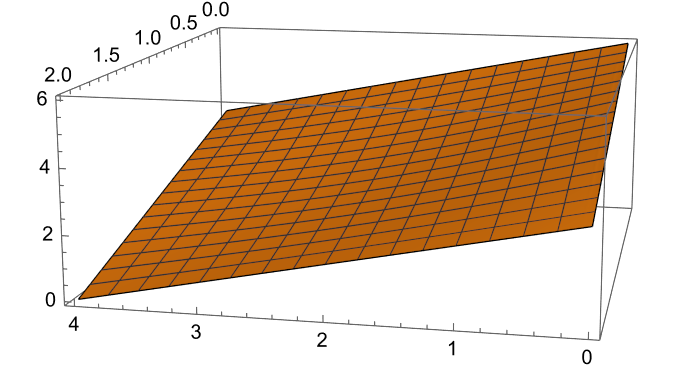
\includegraphics[width=0.7\linewidth]{mytest.png}
	\end{figure}
	\newpage
	\begin{thebibliography}{1}
		\bibitem{galanin} \textit{Галанин М.П., Савенков Е.Б.} Методы численного анализа математических\\ моделей. М.: Изд-во МГТУ им. Н.Э. Баумана,	2010. 592 с.
		\bibitem{kalitkin} \textit{Калиткин Н.Н.} Численные методы. М.: Наука, 1978. 512 с.
		
		
	\end{thebibliography}
	
	
\end{document}
